% Options for packages loaded elsewhere
% Options for packages loaded elsewhere
\PassOptionsToPackage{unicode}{hyperref}
\PassOptionsToPackage{hyphens}{url}
\PassOptionsToPackage{dvipsnames,svgnames,x11names}{xcolor}
%
\documentclass[
  10t,
]{article}
\usepackage{xcolor}
\usepackage{amsmath,amssymb}
\setcounter{secnumdepth}{-\maxdimen} % remove section numbering
\usepackage{iftex}
\ifPDFTeX
  \usepackage[T1]{fontenc}
  \usepackage[utf8]{inputenc}
  \usepackage{textcomp} % provide euro and other symbols
\else % if luatex or xetex
  \usepackage{unicode-math} % this also loads fontspec
  \defaultfontfeatures{Scale=MatchLowercase}
  \defaultfontfeatures[\rmfamily]{Ligatures=TeX,Scale=1}
\fi
\usepackage{lmodern}
\ifPDFTeX\else
  % xetex/luatex font selection
\fi
% Use upquote if available, for straight quotes in verbatim environments
\IfFileExists{upquote.sty}{\usepackage{upquote}}{}
\IfFileExists{microtype.sty}{% use microtype if available
  \usepackage[]{microtype}
  \UseMicrotypeSet[protrusion]{basicmath} % disable protrusion for tt fonts
}{}
\makeatletter
\@ifundefined{KOMAClassName}{% if non-KOMA class
  \IfFileExists{parskip.sty}{%
    \usepackage{parskip}
  }{% else
    \setlength{\parindent}{0pt}
    \setlength{\parskip}{6pt plus 2pt minus 1pt}}
}{% if KOMA class
  \KOMAoptions{parskip=half}}
\makeatother
% Make \paragraph and \subparagraph free-standing
\makeatletter
\ifx\paragraph\undefined\else
  \let\oldparagraph\paragraph
  \renewcommand{\paragraph}{
    \@ifstar
      \xxxParagraphStar
      \xxxParagraphNoStar
  }
  \newcommand{\xxxParagraphStar}[1]{\oldparagraph*{#1}\mbox{}}
  \newcommand{\xxxParagraphNoStar}[1]{\oldparagraph{#1}\mbox{}}
\fi
\ifx\subparagraph\undefined\else
  \let\oldsubparagraph\subparagraph
  \renewcommand{\subparagraph}{
    \@ifstar
      \xxxSubParagraphStar
      \xxxSubParagraphNoStar
  }
  \newcommand{\xxxSubParagraphStar}[1]{\oldsubparagraph*{#1}\mbox{}}
  \newcommand{\xxxSubParagraphNoStar}[1]{\oldsubparagraph{#1}\mbox{}}
\fi
\makeatother

\usepackage{color}
\usepackage{fancyvrb}
\newcommand{\VerbBar}{|}
\newcommand{\VERB}{\Verb[commandchars=\\\{\}]}
\DefineVerbatimEnvironment{Highlighting}{Verbatim}{commandchars=\\\{\}}
% Add ',fontsize=\small' for more characters per line
\usepackage{framed}
\definecolor{shadecolor}{RGB}{248,248,248}
\newenvironment{Shaded}{\begin{snugshade}}{\end{snugshade}}
\newcommand{\AlertTok}[1]{\textcolor[rgb]{0.94,0.16,0.16}{#1}}
\newcommand{\AnnotationTok}[1]{\textcolor[rgb]{0.56,0.35,0.01}{\textbf{\textit{#1}}}}
\newcommand{\AttributeTok}[1]{\textcolor[rgb]{0.13,0.29,0.53}{#1}}
\newcommand{\BaseNTok}[1]{\textcolor[rgb]{0.00,0.00,0.81}{#1}}
\newcommand{\BuiltInTok}[1]{#1}
\newcommand{\CharTok}[1]{\textcolor[rgb]{0.31,0.60,0.02}{#1}}
\newcommand{\CommentTok}[1]{\textcolor[rgb]{0.56,0.35,0.01}{\textit{#1}}}
\newcommand{\CommentVarTok}[1]{\textcolor[rgb]{0.56,0.35,0.01}{\textbf{\textit{#1}}}}
\newcommand{\ConstantTok}[1]{\textcolor[rgb]{0.56,0.35,0.01}{#1}}
\newcommand{\ControlFlowTok}[1]{\textcolor[rgb]{0.13,0.29,0.53}{\textbf{#1}}}
\newcommand{\DataTypeTok}[1]{\textcolor[rgb]{0.13,0.29,0.53}{#1}}
\newcommand{\DecValTok}[1]{\textcolor[rgb]{0.00,0.00,0.81}{#1}}
\newcommand{\DocumentationTok}[1]{\textcolor[rgb]{0.56,0.35,0.01}{\textbf{\textit{#1}}}}
\newcommand{\ErrorTok}[1]{\textcolor[rgb]{0.64,0.00,0.00}{\textbf{#1}}}
\newcommand{\ExtensionTok}[1]{#1}
\newcommand{\FloatTok}[1]{\textcolor[rgb]{0.00,0.00,0.81}{#1}}
\newcommand{\FunctionTok}[1]{\textcolor[rgb]{0.13,0.29,0.53}{\textbf{#1}}}
\newcommand{\ImportTok}[1]{#1}
\newcommand{\InformationTok}[1]{\textcolor[rgb]{0.56,0.35,0.01}{\textbf{\textit{#1}}}}
\newcommand{\KeywordTok}[1]{\textcolor[rgb]{0.13,0.29,0.53}{\textbf{#1}}}
\newcommand{\NormalTok}[1]{#1}
\newcommand{\OperatorTok}[1]{\textcolor[rgb]{0.81,0.36,0.00}{\textbf{#1}}}
\newcommand{\OtherTok}[1]{\textcolor[rgb]{0.56,0.35,0.01}{#1}}
\newcommand{\PreprocessorTok}[1]{\textcolor[rgb]{0.56,0.35,0.01}{\textit{#1}}}
\newcommand{\RegionMarkerTok}[1]{#1}
\newcommand{\SpecialCharTok}[1]{\textcolor[rgb]{0.81,0.36,0.00}{\textbf{#1}}}
\newcommand{\SpecialStringTok}[1]{\textcolor[rgb]{0.31,0.60,0.02}{#1}}
\newcommand{\StringTok}[1]{\textcolor[rgb]{0.31,0.60,0.02}{#1}}
\newcommand{\VariableTok}[1]{\textcolor[rgb]{0.00,0.00,0.00}{#1}}
\newcommand{\VerbatimStringTok}[1]{\textcolor[rgb]{0.31,0.60,0.02}{#1}}
\newcommand{\WarningTok}[1]{\textcolor[rgb]{0.56,0.35,0.01}{\textbf{\textit{#1}}}}

\usepackage{longtable,booktabs,array}
\usepackage{calc} % for calculating minipage widths
% Correct order of tables after \paragraph or \subparagraph
\usepackage{etoolbox}
\makeatletter
\patchcmd\longtable{\par}{\if@noskipsec\mbox{}\fi\par}{}{}
\makeatother
% Allow footnotes in longtable head/foot
\IfFileExists{footnotehyper.sty}{\usepackage{footnotehyper}}{\usepackage{footnote}}
\makesavenoteenv{longtable}
\usepackage{graphicx}
\makeatletter
\newsavebox\pandoc@box
\newcommand*\pandocbounded[1]{% scales image to fit in text height/width
  \sbox\pandoc@box{#1}%
  \Gscale@div\@tempa{\textheight}{\dimexpr\ht\pandoc@box+\dp\pandoc@box\relax}%
  \Gscale@div\@tempb{\linewidth}{\wd\pandoc@box}%
  \ifdim\@tempb\p@<\@tempa\p@\let\@tempa\@tempb\fi% select the smaller of both
  \ifdim\@tempa\p@<\p@\scalebox{\@tempa}{\usebox\pandoc@box}%
  \else\usebox{\pandoc@box}%
  \fi%
}
% Set default figure placement to htbp
\def\fps@figure{htbp}
\makeatother





\setlength{\emergencystretch}{3em} % prevent overfull lines

\providecommand{\tightlist}{%
  \setlength{\itemsep}{0pt}\setlength{\parskip}{0pt}}



 


\makeatletter
\@ifpackageloaded{tcolorbox}{}{\usepackage[skins,breakable]{tcolorbox}}
\@ifpackageloaded{fontawesome5}{}{\usepackage{fontawesome5}}
\definecolor{quarto-callout-color}{HTML}{909090}
\definecolor{quarto-callout-note-color}{HTML}{0758E5}
\definecolor{quarto-callout-important-color}{HTML}{CC1914}
\definecolor{quarto-callout-warning-color}{HTML}{EB9113}
\definecolor{quarto-callout-tip-color}{HTML}{00A047}
\definecolor{quarto-callout-caution-color}{HTML}{FC5300}
\definecolor{quarto-callout-color-frame}{HTML}{acacac}
\definecolor{quarto-callout-note-color-frame}{HTML}{4582ec}
\definecolor{quarto-callout-important-color-frame}{HTML}{d9534f}
\definecolor{quarto-callout-warning-color-frame}{HTML}{f0ad4e}
\definecolor{quarto-callout-tip-color-frame}{HTML}{02b875}
\definecolor{quarto-callout-caution-color-frame}{HTML}{fd7e14}
\makeatother
\makeatletter
\@ifpackageloaded{caption}{}{\usepackage{caption}}
\AtBeginDocument{%
\ifdefined\contentsname
  \renewcommand*\contentsname{Table of contents}
\else
  \newcommand\contentsname{Table of contents}
\fi
\ifdefined\listfigurename
  \renewcommand*\listfigurename{List of Figures}
\else
  \newcommand\listfigurename{List of Figures}
\fi
\ifdefined\listtablename
  \renewcommand*\listtablename{List of Tables}
\else
  \newcommand\listtablename{List of Tables}
\fi
\ifdefined\figurename
  \renewcommand*\figurename{Figure}
\else
  \newcommand\figurename{Figure}
\fi
\ifdefined\tablename
  \renewcommand*\tablename{Table}
\else
  \newcommand\tablename{Table}
\fi
}
\@ifpackageloaded{float}{}{\usepackage{float}}
\floatstyle{ruled}
\@ifundefined{c@chapter}{\newfloat{codelisting}{h}{lop}}{\newfloat{codelisting}{h}{lop}[chapter]}
\floatname{codelisting}{Listing}
\newcommand*\listoflistings{\listof{codelisting}{List of Listings}}
\makeatother
\makeatletter
\makeatother
\makeatletter
\@ifpackageloaded{caption}{}{\usepackage{caption}}
\@ifpackageloaded{subcaption}{}{\usepackage{subcaption}}
\makeatother
\usepackage{bookmark}
\IfFileExists{xurl.sty}{\usepackage{xurl}}{} % add URL line breaks if available
\urlstyle{same}
\hypersetup{
  pdftitle={Artificial Intelligence for Academic Integrity (AI4AI)},
  pdfauthor={AJ Smit},
  colorlinks=true,
  linkcolor={blue},
  filecolor={blue},
  citecolor={blue},
  urlcolor={blue},
  pdfcreator={LaTeX via pandoc}}


\title{Artificial Intelligence for Academic Integrity (AI4AI)}
\author{AJ Smit}
\date{2025-03-17}
\begin{document}
\maketitle


\section{Introduction}\label{introduction}

Although Generative Artificial Intelligence (AI) has been available to
the research community since the late 2010s, a cutting-edge version of
the software in the form of ChatGPT was released for widespread
consumption in November 2022. \href{https://chat.openai.com/}{OpenAI} is
the most well-known of these AI platforms, but the landscape is dotted
with other similar models such as Anthropic's Claude, Google's Gemini,
Perplexity, and DeepSeek. The moniker ``GPT'' stands for Generative
Pre-trained Transformer and is core to all these platforms. They come in
free versions and paid versions with enhanced capabilities. Together,
they are a class of neural networks called Large Language Models (LLMs),
and their attraction is their ability to process natural language in a
manner that makes them seem intelligent. They can do with ease many of
the tasks that academics and students deal with.

Since their widespread public release in 2022, LLMs have been undergoing
exponential development such that the frontier models with ``Deep
Research'' capabilities are now able to perform advanced reasoning on
par with (or exceeding in some cases) what one would expect of PhD-level
individuals. Clearly, the consequences for academia are immense and
paradigm-shifting. Today's cutting-edge models are more than simply
language processors, as they have become increasingly integrated into
different computational modalities (the so-called multi-modal models),
which has broadened their field of application to code, data analysis,
image and video, spoken language processing, and so forth. Some models
such as \href{https://www.thesisai.io}{Thesis AI} exist solely to meet
the needs of postgraduates, and others such as
\href{https://scholarai.io}{Scholar AI},
\href{https://elicit.com}{Elicit}, and
\href{https://consensus.app}{Consensus} were made for academia more
generally for tasks such as literature searches, summaries, and
generating deep reviews. The explosion of interest reflects how the
applications and uses of AI are rapidly developing, including being used
by under- and postgraduate students. As educators, we must continue
ensuring that our teaching practices and module content provide students
with the knowledge and skills they need to navigate the world of AI
within the ever-changing scope of academic integrity.

In fact, the core definition of what constitutes academic integrity has
come into question.

\section{AI in Academia}\label{ai-in-academia}

Students and educators face certain threats, but we need to also
acknowledge the many opportunities. Let's explore these:

We probably need guides or policies for the key academic activities,
including for academic staff (teaching, learning, and research),
undergraduate students, postgraduate students and researchers. below,
I'll briefly outline some ideas currently bouncing around the BCB
department.

\subsection{Educators}\label{educators}

Opportunities include:

\begin{itemize}
\tightlist
\item
  Develop syllabi and curricula.
\item
  Create personalised learning paths for students based on their
  individual progress and learning styles.
\item
  Produce lecture materials (slides, notes, transcripts of lectures, all
  aspects of lecture content generation).
\item
  Sketch lesson plans, differentiate worksheets, and generate exemplar
  answers -- can cut weekly preparation time by almost one-third and
  free bandwidth for in-person mentorship.
\item
  Combine AI with VR technology to create immersive educational
  simulations.
\item
  Setting of assessment questions together with rubrics and model
  answers.
\item
  Applying AI to analyse learning patterns and provide actionable
  insights to optimise instruction.
\item
  Developing module-specific intelligent tutors for self-paced assisted
  learning and self-assessments (through a Socratic prompt engine) --
  done right, this could offer opportunities for driving higher-order
  learning across the syllabus).
\item
  Using AI-based platforms to develop exercises around specific skills,
  such as coding or language proficiency.
\item
  Utilising AI's natural language processing capabilities for tasks like
  automated language translation, question-answering systems, and text
  analysis (useful for teaching non-native English speakers).
\item
  New forms of assessment, such as assigning students the task of
  critiquing LLM output for logical fallacies, biases, and factual
  accuracy.
\item
  AI-assisted grading that draws on LLMs fine-tuned to module-specific
  content and detailed rubric criteria; such assessments can parse
  argument structure, navigate lexical anomalies, and flag outlier
  submissions (for human intervention), and reduce marking hours
  (helpful for large classes). Such feedback can increase the
  granularity of timely, actionable feedback that students receive.
\item
  Utilising AI for automating administrative tasks such as scheduling,
  and record-keeping.
\item
  Develop module-specific AI guidelines and policies to build upon a
  faculty-wide Basic AI Literacy core module.
\end{itemize}

The above opportunities necessitate redeveloping testing logistics and
adapting the ontology of evidence.

I observe that some colleagues invest excessive confidence in AI
detection tools. This amplifies the probability that students face
unfounded accusations of academic dishonesty. We must always keep
academic integrity central in our pedagogical considerations, but
adopting punitive measures will more likely force dishonest practices
into concealment rather than develop the critical competencies our
students require for their intellectual futures.

\subsection{Students}\label{students}

What are the threats of AI to students? These topics must feature in a
core ``Basic AI Literacy'' course early on in students' academic
careers:

\begin{itemize}
\tightlist
\item
  Academic integrity in the age of AI.
\item
  A topology of AI: the basics.
\item
  The diversity of AI tools.
\item
  What is knowledge and where does it come from?
\item
  What are the risks to privacy?
\item
  How to be aware of and guard against inaccuracies and biases.
\item
  Hallucinations, including the generating fictitious references (always
  engage directly with the primary references via established methods
  such as Google Scholar and Scopus and the like) \ldots{} although,
  some specialist AI reference discovery tools are now available, but
  typically a subscription is necessary for advanced features.
\item
  AI model training and release cycles.
\item
  The ethics of AI ``knowledge''.
\item
  The problem with ghost writing (e.g.~essays).
\item
  ``Temptations'' during open-book assessments and assignments.
\item
  Deeper and updated discussions around plagiarism (requiring redefining
  what it means to plagiarise).
\item
  The dangers of excessive reliance on AI and the consequences for
  students failing to acquire ``personal knowledge.''
\item
  The consequences of being incapable to problem solve and apply
  critical thinking.
\item
  The false belief that AI is infallible: what happens when students
  accept LLM answers as the final word in believable, seemingly
  factually correct answers to almost any question? This leads to a loss
  of critical questioning and scepticism. Always validate all AI
  generated content and ground within the peer-reviewed (or vetted)
  knowledge base.
\item
  The dangers and ethics of specialist academic oriented AI tools such
  as Thesis AI.
\end{itemize}

What opportunities does AI offer students?

\begin{itemize}
\tightlist
\item
  The importance of prompts: the dangers of the untenable expectations
  ``10 words in, 1000 words out'' vs.~``1000 words in, 1000 words out''
  .
\item
  Dialogic tutors (e.g., Socratic method and personal knowledge
  assessors).
\item
  Deeper research and enhancing the ability to use critical thinking to
  create meaningful knowledge from information; students must be able to
  identify what information is required to complete their assignments or
  assessments, and then evaluate this information and communicate it in
  an ethical and legal manner, including acknowledgement and citation of
  all sources, including AI.
\item
  Done correctly, easy access to vast knowledge in a language accessible
  to individuals at almost any level of foundational knowledge.
\item
  The ability to deal with more-and-more complex problems.
\item
  Fast-tracking the research process.
\item
  Collaborator and research partner (bouncing ideas and feedback).
\item
  Mock peer-reviewers or thesis examiners (anticipate problems before
  they arise).
\end{itemize}

\section{The Way Forward}\label{the-way-forward}

We may opt to avoid AI altogether by reverting to in-person and other
forms of ``traditional'' assessment. But this ``solution'' is
problematic as it creates as many challenges as it purports to solve.
Moreover, given the new technology landscape and our modern mode of
engaging with information and knowledge, we move away from authentic
assessment; that is, assessment reflecting today's technology landscape.

Another approach often taken in response to AI encroaching more and more
on our lives is to try and outrun it. The problem with this approach is
that AI is advancing so rapidly that we will never catch this advancing
target. Such pre-emptive actions are also likely to be too
time-consuming to be practical.

The most reasonable solution is therefore to embrace AI, adapt to the
new opportunities, and integrate AI into the curriculum at strategic
points. The most critical requirement is that a Basic AI Literacy module
must be offered to all students at the start of their academic careers.
Some core discipline-specific modules can then teach those AI skills
that will become indispensable tools of the discipline. For example,
many scientific modules require a well-developed coding toolkit, and in
the right hands, AI will become part of analytical workflows. Similarly,
skills specific to literature searches and reviews, writing, reviewing,
and other scholarly practices can be taught when required.

\section{A Taxonomy of AI}\label{a-taxonomy-of-ai}

\subsection{I. Artificial Intelligence
(AI)}\label{i.-artificial-intelligence-ai}

The broad, interdisciplinary field focussed on building machines that
perform tasks requiring ``intelligence'' as done by people: reasoning,
learning, perception, language use, decision-making.

Encompasses:

\begin{itemize}
\tightlist
\item
  Symbolic AI (rule-based systems, logic programming)
\item
  Probabilistic AI (Bayesian models, Markov decision processes)
\item
  \textbf{Machine Learning} (data-driven statistical modeling)
\end{itemize}

\subsection{II. Machine Learning (ML)}\label{ii.-machine-learning-ml}

A subfield of AI focused on algorithms that learn from data to improve
their performance without being explicitly programmed for every task.

Subtypes:

\begin{itemize}
\tightlist
\item
  \textbf{Supervised Learning} --- learns from labelled data (e.g.,
  regression, classification)
\item
  \textbf{Unsupervised Learning} --- finds patterns in unlabelled data
  (e.g., clustering, dimensionality reduction)
\item
  \textbf{Reinforcement Learning} --- learns through interaction with an
  environment via rewards/punishments
\item
  \textbf{Deep Learning} --- a class of machine learning using
  multi-layered neural networks
\end{itemize}

\subsection{III. Neural Networks}\label{iii.-neural-networks}

A family of algorithms inspired by the human brain, composed of layers
of interconnected units (``neurons'') that can approximate complex
functions.

Includes:

\begin{itemize}
\tightlist
\item
  Feedforward Networks
\item
  Convolutional Neural Networks (CNNs) --- often used for images
\item
  Recurrent Neural Networks (RNNs) --- time-sequence data
\item
  \textbf{Transformer Networks} --- the architecture underpinning modern
  LLMs
\end{itemize}

\subsection{IV. Large Language Models
(LLMs)}\label{iv.-large-language-models-llms}

Very large nd dense neural networks (typically transformer-based)
trained on vast (internet-sized) amounts of text data to learn patterns,
structures, and nuances of language which enables them to perform tasks
such as translation, summarisation, question answering, and more. Their
purpuse is on ``understanding'' and generating human language.

Features: - Built on transformer architecture - Typically have billions
of parameters - Trained on datasets ranging from books, websites, code
repositories - Capable of few-shot, zero-shot, and in-context learning -
Output is generative: new text, answers, translations, summaries

LLMs are often used in applications like chatbots, virtual assistants,
content generation, and more. They can also be fine-tuned for specific
tasks or domains.

\subsection{V. GPT (Generative Pretrained Transformer)
Models}\label{v.-gpt-generative-pretrained-transformer-models}

A specific family of LLMs (developed by OpenAI), built on a decoder-only
transformer architecture. Trained with next-token prediction on
internet-scale text.

Examples:

\begin{itemize}
\tightlist
\item
  Popularised by OpenAI, e.g., GPT-2, GPT-3, GPT-4, GPT-4o
\item
  Distinctive for their use in chat interfaces (e.g., ChatGPT)
\item
  Fine-tuned for tasks like conversation, instruction following,
  summarisation, reasoning
\end{itemize}

\subsection{VI. What Can the Models
Do?}\label{vi.-what-can-the-models-do}

These define what kind of content or data the AI can work with. Often,
these modalities are blended in multimodal models, but the categories
remain conceptually distinct.

Text:

\begin{itemize}
\tightlist
\item
  Summarisation, translation, paraphrasing, answering questions, text
  classification
\item
  Models: GPT, Gemini, Claude, etc.
\end{itemize}

Code:

\begin{itemize}
\tightlist
\item
  Code generation, debugging, refactoring, documentation
\item
  Models: Copilot, Codex, AlphaCode, CodeLlama
\end{itemize}

Image:

\begin{itemize}
\tightlist
\item
  Image generation, recognition, captioning, segmentation
\item
  Models: DALL·E, Midjourney, Stable Diffusion, CLIP
\end{itemize}

Voice / Audio:

\begin{itemize}
\tightlist
\item
  Speech recognition (ASR), speech synthesis (TTS), voice translation
\item
  Models: Whisper, VALL-E, AudioLM
\end{itemize}

Multimodal (Text + Image + Audio + Video):

\begin{itemize}
\tightlist
\item
  Interacting across multiple data types, e.g., describing an image,
  reading from a graph, watching a video and answering questions
\item
  Models: GPT-4o, Gemini 1.5, Claude 3 with vision, Flamingo
\end{itemize}

\begin{enumerate}
\def\labelenumi{\Roman{enumi}.}
\setcounter{enumi}{6}
\tightlist
\item
  Summary Diagram (Outline Form)
\end{enumerate}

\begin{Shaded}
\begin{Highlighting}[]
\NormalTok{Artificial Intelligence (AI)}
\NormalTok{│}
\NormalTok{├── Symbolic AI}
\NormalTok{├── Probabilistic AI}
\NormalTok{└── Machine Learning (ML)}
\NormalTok{    │}
\NormalTok{    ├── Supervised / Unsupervised / Reinforcement Learning}
\NormalTok{    └── Deep Learning}
\NormalTok{        └── Neural Networks}
\NormalTok{            └── Transformer Architecture}
\NormalTok{                └── Large Language Models (LLMs)}
\NormalTok{                    └── GPT Models}
\NormalTok{                        └── GPT{-}4, GPT{-}4o, etc.}

\NormalTok{Modal Competencies:}
\NormalTok{{-} Text: GPT, Claude, T5}
\NormalTok{{-} Code: Codex, CodeLlama}
\NormalTok{{-} Images: DALL·E, Stable Diffusion}
\NormalTok{{-} Voice: Whisper, AudioLM}
\NormalTok{{-} Multimodal: GPT{-}4o, Gemini, Claude 3}
\end{Highlighting}
\end{Shaded}

LLMs support academic work in various ways. In this workshop, I will
explore some of the ways in which the GPT models can be used in our
academic research whilst keeping an eye on academic integrity.

LLMs have their distinct ``personalities'', but they also have various
personalisation options to help ``humanise'' their writing. In this
workshop, we will go over the strengths and weaknesses of all these
models, and we will look at how to customise them in ways that will
improve academic integrity and bring them in line with how people
\emph{actually} write.

Many new AI models appear each day, some with the needs of academics in
mind. For example, \href{https://elicit.com/}{Elicit},
\href{https://www.researchrabbit.ai/}{ResearchRabbit}, and
\href{https://www.scholarcy.com/}{Scholarcy} also support the type and
style of writing we do. Many also help us make sense of a bewildering
body of peer-reviewed research papers. I'll spend less time with these,
but the basic principles that apply to the GPTs developed for general
consumption work here too.

\section{LLM Models}\label{llm-models}

A variety of LLM models are available for use in academia. These models
include:

\begin{itemize}
\tightlist
\item
  \href{https://openai.com/}{\textbf{OpenAI}}

  \begin{itemize}
  \tightlist
  \item
    \textbf{GPT-4o-mini}\footnote{``o'' models are referred to as
      ``reasoning models''.}
  \item
    GPT-o1
  \item
    GPT-o1-mini
  \item
    GPT-o1-mini-high
  \item
    \textbf{GPT-o3-mini}
  \item
    \textbf{GPT-4o}
  \item
    GPT 4.5
  \item
    Has ``Customise ChatGPT'' option
  \end{itemize}
\item
  \href{https://www.anthropic.com/}{\textbf{Anthropic}}

  \begin{itemize}
  \tightlist
  \item
    \textbf{Claude 3.7 Sonnet}
  \item
    \textbf{Claude 3.5 Haiku}
  \item
    Two thinking modes: \textbf{Normal} and Extended
  \item
    Has ``Projects'' and ``Styles'' for customisation
  \end{itemize}
\item
  \href{https://one.google.com/intl/en_za/about/ai-premium/}{\textbf{Google
  Gemini}}

  \begin{itemize}
  \tightlist
  \item
    \textbf{Google Scholar}
  \item
    \textbf{2.0 Flash}
  \item
    \textbf{2.0 Flash Thinking}
  \item
    Gemini Advanced
  \item
    Deep Research
  \item
    Experimental models
  \item
    2.0 Pro
  \item
    \textbf{\href{https://notebooklm.google.com/}{NotebookLM}} (built on
    Gemini)
  \item
    NotebookLM Plus
  \item
    Option to use ``Gems''
  \end{itemize}
\item
  \href{https://manus.im/}{Manus}
\item
  \href{https://elicit.com}{Elicit}
\item
  \href{https://scholarai.io/}{Scholar.AI}
\item
  \href{https://deepseek.ai/}{DeepSeek}
\item
  \href{https://www.perplexity.ai/}{Perplexity}
\item
  \href{https://consensus.app/}{Consensus}
\item
  \href{https://www.thesisai.io/}{Thesis.AI}
\item
  \href{https://github.com/features/copilot}{GitHub Copilot}, available
  to all academic users with a GitHub account. It is accessible via the
  RStudio interface.
\end{itemize}

\subsection{Code Editor Integrations}\label{code-editor-integrations}

\begin{itemize}
\tightlist
\item
  \href{https://github.com/features/copilot}{Copilot}
\item
  \href{https://www.cursor.com}{Cursor}
\item
  \href{https://windsurf.com}{Windsurf}
\item
  \href{https://lovable.dev}{Lovable}
\item
  \href{https://firebase.google.com}{Google Firebase}
\item
  \href{https://www.anthropic.com/claude-code}{Anthropic Code}
\item
  \href{https://posit.co/products/open-source/rstudio/}{RStudio}
\end{itemize}

\subsection{Academic Use: Teaching and
Learning}\label{academic-use-teaching-and-learning}

\begin{itemize}
\tightlist
\item
  \href{https://www.mindjoy.com}{Mindjoy}
\item
  \href{https://notebooklm.google/}{NotebookLM}
\end{itemize}

\section{The Importance of Prompts}\label{the-importance-of-prompts}

Prompts are important in guiding the AI to generate the desired output.
Well-crafted prompts allow you use AI to help you improve the amount of
signal you have amongst all the noise.

The better the prompt, the better the output. Asking insightful,
well-informed, detailed, and descriptive questions will lead to better
results. Aksing questions as a 10-year old would will lead to poor
results. In AI, there really is such a thing as a dumb question! Simply
put, there are two approaches to prompting:

\begin{itemize}
\tightlist
\item
  enter 10 words in and expect a thousand words out, and
\item
  enter 1000 words in and expect a thousand words out.
\end{itemize}

In this part of the workshop, I will discuss the importance of prompts
and how to ask good questions.

\subsection{Use Markdown to structure your
prompts}\label{use-markdown-to-structure-your-prompts}

When writing prompts, use markdown to structure your text. Use headings,
lists, and other formatting options to make your prompts clear and easy
to read. This will help the AI understand your request better and
generate more relevant responses.

\begin{longtable}[]{@{}
  >{\raggedright\arraybackslash}p{(\linewidth - 4\tabcolsep) * \real{0.0588}}
  >{\raggedright\arraybackslash}p{(\linewidth - 4\tabcolsep) * \real{0.2574}}
  >{\raggedright\arraybackslash}p{(\linewidth - 4\tabcolsep) * \real{0.6838}}@{}}
\toprule\noalign{}
\begin{minipage}[b]{\linewidth}\raggedright
Symbol
\end{minipage} & \begin{minipage}[b]{\linewidth}\raggedright
Meaning (Translated)
\end{minipage} & \begin{minipage}[b]{\linewidth}\raggedright
Use Case / Additional Notes
\end{minipage} \\
\midrule\noalign{}
\endhead
\bottomrule\noalign{}
\endlastfoot
\texttt{\#} & Organises information & Often used as a heading marker
(like Markdown). Helps segment prompts into sections. \\
\texttt{*} & Emphasises or creates lists & Useful for bullet points,
emphasis, or making instructions clearer. \\
\texttt{\{\}} & User input variable & Placeholder for custom input
(e.g., \texttt{\{topic\}}), great for reusable prompt templates. \\
\texttt{{[}{]}} & Optional elements or choices & Indicates optional
words or parameters, or choice selection (e.g.,
\texttt{{[}formal/informal{]}}). \\
\texttt{\textless{}\textgreater{}} & Interchangeable or dynamic content
& Used to represent something that will be substituted dynamically. Less
common than \texttt{\{\}}. \\
\texttt{-} & Creates bullet or step list & Used to structure steps or
items cleanly, especially when writing multi-part answers. \\
\end{longtable}

\subsection{Setting up your writing style and prior
expectations}\label{setting-up-your-writing-style-and-prior-expectations}

An example pre-configuration of the AI for your writing style and prior
expectations is as follows:

\begin{tcolorbox}[enhanced jigsaw, left=2mm, colframe=quarto-callout-note-color-frame, arc=.35mm, colback=white, leftrule=.75mm, toprule=.15mm, bottomrule=.15mm, rightrule=.15mm, breakable, opacityback=0]
\begin{minipage}[t]{5.5mm}
\textcolor{quarto-callout-note-color}{\faInfo}
\end{minipage}%
\begin{minipage}[t]{\textwidth - 5.5mm}

\vspace{-3mm}\textbf{ChatGPT profile}\vspace{3mm}

Think step-by-step, showing reasoning for complex problems.

Break down complex tasks and ask clarifying questions, if needed. Ask me
if you are unclear.

Aim to be scholarly, confident, and analytical, appealing to readers
accustomed to advanced academic dialogue. Maintain a poised authority,
weaving scientific depth without slipping into empty verbosity. While
the vocabulary reflects complexity -- e.g.~``epistemic,'' ``conceptual
ordering,'' ``structured inference,'' and ``rigorous standard'' -- do
not use jargon for its own sake. Emphasise clarity that respects the
reader's intelligence and allows concepts to resonate without
condescension.

Let the sentence structure shift between long, layered forms that
contextualise, define, and critically engage, and shorter, sharper
sentences that reinforce key arguments and points. Use a variety of
clauses, parenthetical asides, and em-dashes to give the writing a
dynamic flow. This rhythmic variation and precise diction shape a voice
that rewards a close, attentive reading.

Some phrases recur to define the analytical approach, e.g.,
``particularly,'' ``structured inference,'' ``conceptual groundwork,''
``rigorous standard,'' ``systematic reasoning,'' ``intellectual
milieu,'' and ``distinguish signal from noise.'' Constructions like
``laid the foundation for,'' ``conceptual leap,'' and ``philosophical
tradition'' emphasise historical continuity and highlight how earlier
ideas inform contemporary discourse.

Avoid these words: particularly, crucial(ly), essential, holistic,
especially, challenge(s), sophisticated, ensuring/ensure, profound,
remarkable, nuanced, emerge(s), questioning, nudge(s), robust, ``stand
out,'' ``by acknowledging,'' ``It's a reminder,'' ``In summary.''

Aim for a
\href{https://en.wikipedia.org/wiki/Gunning_fog_index}{Gunning-Fog
index} above 23, and use British English.

Avoid words that flatten complexity or imply hollow emphasis. Rely on
carefully chosen terms that reflect a style suited to readers ready to
engage with advanced scholarly thought.

Avoid excessive political correctness, overly polite answers, being
apologetic, or always assuming I am correct. I appreciate being argued
or disagreed with.

I like a detailed, critical analysis. I dislike bullet points (unless
absolutely necessary). I value long-form writing. I dislike formulaic
responses, like paragraphs of equal length --- keep them varied. Avoid
the concluding paragraph starting with ``In summary\ldots{}''. In fact,
avoid these silly summary paragraphs altogether.

\end{minipage}%
\end{tcolorbox}

\subsection{Write detailed prompts}\label{write-detailed-prompts}

Two modes of use:

\begin{itemize}
\item
  10 words in, 1000 words out
\item
  1000 words in, 1000 words out
\item
  Emphasis on ``slow knowledge'' and ``deep thinking''.
\end{itemize}

\begin{tcolorbox}[enhanced jigsaw, left=2mm, colframe=quarto-callout-note-color-frame, arc=.35mm, colback=white, leftrule=.75mm, toprule=.15mm, bottomrule=.15mm, rightrule=.15mm, breakable, opacityback=0]
\begin{minipage}[t]{5.5mm}
\textcolor{quarto-callout-note-color}{\faInfo}
\end{minipage}%
\begin{minipage}[t]{\textwidth - 5.5mm}

Be as verbose and explicit as you can be when writing your prompts.
Provide all the necessary background information, and be specific about
what you want the AI to do. For example, instead of asking ``What is the
impact of climate change on marine ecosystems?'', you could ask ``Can
you provide a detailed analysis of how climate change affects marine
ecosystems, including changes in temperature, ocean acidification, and
shifts in species distribution? Please include recent research findings
and examples from different regions.'' This will give you a reasonable
chance of getting a more detailed and relevant response.

But to be even more effective, try constructing a prompt like this one:

\subsection{Example 1}\label{example-1}

A recent method adapted from the marine heatwave and marine cold spell
detection methodology integrates high-resolution SST data from multiple
products with wind measurements. The method works by detecting
simultaneous increases in south-easterly winds and corresponding
decreases in SST, which signal the occurrence of upwelling. By
calculating metrics like intensity (magnitude of SST drops), duration
(length of time the event persists), and frequency (how often upwelling
events occur), the authors create a comprehensive tool for evaluating
upwelling dynamics.

The metrics are calculated on the SST data, where an upwelling event
(henceforth `event') is signalled by the drop in SST below a threshold,
i.e.~``If the temperature dropped {[}below{]} the seasonally varying
25th percentile of SST for a particular site, we deemed this a
confirmation of the occurrence of an upwelling event at that site.'' So,
an event is detected as TRUE when this drop occurs and persists for a
day or more. I think that more frequent and longer-lasting events will
lower SST during the upwelling season. If, over time (decades),
upwelling events become more frequent and longer lasting, it will be
accompanied by a decadal shift (lowering) in SST.

The paper that developed this methodology studied these upwelling events
in conjunction with ``simultaneous increases in south-easterly winds.''
They did not use wind stress curl, which could be a significant
omission. Could wind stress curl better predict SST and upwelling event
metrics than simply looking at the incidence of south-easterly winds?

Please provide an analysis of the above synopsis of my proposed research
approach. Also, address these questions in the process:

\begin{enumerate}
\def\labelenumi{\arabic{enumi}.}
\tightlist
\item
  How can one use quantile regression to study this problem (i.e., wind
  stress curl as a driver of SST and upwelling event metrics)?
\item
  Is quantile regression the best approach to use?
\item
  How would one determine the threshold below which SST drops when
  signalled as an upwelling event?
\item
  Any other considerations?
\end{enumerate}

\end{minipage}%
\end{tcolorbox}

You could use a synthesis obtained through some deep literature review
as input for developing a structure for your thesis or paper. For
example, using AI output generated earlier, you could ask:

\begin{tcolorbox}[enhanced jigsaw, left=2mm, colframe=quarto-callout-note-color-frame, arc=.35mm, colback=white, leftrule=.75mm, toprule=.15mm, bottomrule=.15mm, rightrule=.15mm, breakable, opacityback=0]
\begin{minipage}[t]{5.5mm}
\textcolor{quarto-callout-note-color}{\faInfo}
\end{minipage}%
\begin{minipage}[t]{\textwidth - 5.5mm}

\vspace{-3mm}\textbf{Example 2}\vspace{3mm}

Please look at this breakdown of knowledge about kelp forests (pasted
below) and suggest only four or five main headings (excluding
subheadings) under which to discuss the status of knoweldge about kelp
globally:

\begin{itemize}
\tightlist
\item
  \textbf{Kelp Forest Ecology} Kelp forests are conspicuously dominated
  by large brown algae and reflect a high degree of biological
  organization. Kelp ecosystems have been the focus of much research
  because of the complexity of biological interactions that structure
  them. Kelp forests provide biogenic habitat that can enhance diversity
  and productivity both locally and over broader spatial scales through
  detrital subsidy.
\item
  \textbf{Kelp Species and Distribution} Kelp species of \emph{Ecklonia
  maxima} and \emph{Laminaria pallida} are commonly found along the west
  coast of southern Africa. \emph{E. maxima} and \emph{L. schinzii} are
  found between the mean low water level and 15 meters below on rocky
  exposed shores, while \emph{L. pallida} occupies areas of lower
  hydrodynamic stress. Molecular tools are being used to test hypotheses
  regarding kelp evolutionary biogeography, in part because kelps have
  sufficient dispersal barriers to enable the study of their evolution
  based on present-day distributions.
\item
  \textbf{Kelp Primary Production and Carbon Cycling} Kelp forests are
  among the most prolific primary producers on the planet, supporting
  productivity per unit area that rivals that of tropical rainforests.
  Kelp forests play a significant role in coastal carbon cycles. Rates
  of carbon assimilation in \emph{Ecklonia radiata} forests can rival
  those of giant kelp forests and \emph{Laminaria} forests.
\item
  \textbf{Kelp-Associated Communities} Numerous faunal species use the
  epiphytic algae associated with the stipe of \emph{Laminaria
  hyperborea} as habitat and a food source. Kelp beds in the southern
  Benguela are associated with about 30 species, many of which are
  fished commercially or recreationally.
\item
  \textbf{Kelp and Fisheries} Changes in kelp density and/or area
  influence the abundance and diversity of associated fisheries. Kelp
  presence and density have an actual effect on associated fisheries.
\item
  \textbf{Kelp Forest Monitoring} Macroalgae are utilized as biological
  indicators of ecosystem health in many monitoring programs worldwide.
  Macroalgae mapping can be carried out through direct observation or by
  indirect methods using remote sensing techniques.
\item
  \textbf{Threats to Kelp Ecosystems} Factors such as climate change,
  overfishing, and invasive species threaten kelp forest ecosystems.
  Darkening in coastal seas associated with increased turbidity results
  in both reduced biomass and depth distribution, and lower productivity
  of \emph{E. radiata}.
\end{itemize}

\textbf{Gaps in Knowledge and Future Research Directions:}

\begin{itemize}
\tightlist
\item
  \textbf{Fate of fixed carbon} A comprehensive understanding of the
  fate of fixed carbon in kelp forests is lacking. Future research
  should focus on the mechanisms of transport, decomposition,
  re-mineralization and burial of kelp-derived organic matter and how
  these may be impacted by anthropogenic- and climate- related changes
  in the environment.
\item
  \textbf{Kelp-fisheries interactions} There are methodological,
  geographical, and logistical gaps that should be filled in order to
  get a broader understanding of interactions between kelp beds and
  fisheries.
\item
  \textbf{South African Kelp Ecosystems} Since the Kelp Bed Ecology
  Programme of the 1970s and 1980s, there has been no concentrated
  research effort afforded to South African kelp ecosystems. Future
  research directions are likely to be centered around the impacts of
  climate change, overfishing and invasive species on kelp forest
  ecosystems.
\item
  \textbf{Harmonization of Marine Macroalgal Monitoring} There is a need
  to harmonize marine macroalgal monitoring, identifying common metrics
  and approaches in sampling design, field measurements, taxonomic
  resolution and data management, in order to develop standardized
  procedures which may allow data obtained to be compared.
\end{itemize}

\end{minipage}%
\end{tcolorbox}

Use AI to generate some synthetic data which you may use to develop,
test, and implement an unknown statistical method. Again, giving it a
full, detailed background to start its reasoning from will get you much
further:

\begin{tcolorbox}[enhanced jigsaw, left=2mm, colframe=quarto-callout-note-color-frame, arc=.35mm, colback=white, leftrule=.75mm, toprule=.15mm, bottomrule=.15mm, rightrule=.15mm, breakable, opacityback=0]
\begin{minipage}[t]{5.5mm}
\textcolor{quarto-callout-note-color}{\faInfo}
\end{minipage}%
\begin{minipage}[t]{\textwidth - 5.5mm}

\vspace{-3mm}\textbf{Example 3}\vspace{3mm}

\textbf{Your initial prompt:} We can measure algal nutrient uptake rates
using two types of experiments: multiple flask experiments and
perturbation experiments. The fundamental concept underlying both
methods is to introduce a known quantity of nutrients (termed the
substrate) into a flask or a series of flasks and then measure the rate
of nutrient uptake (\(V\)) at different substrate concentrations
(\([S]\)). We calculate the nutrient uptake rate as the change in
nutrient concentration in the flask over a predefined time interval
(\(V = \Delta [S]/\Delta t\)). Consequently, both experiments generate
data that relate the nutrient uptake rate to the corresponding substrate
concentration. The primary difference between the two methods lies in
the experimental setup and the data analysis.

In the \textbf{multiple flask method}, we prepare a series of flasks,
each containing a different initial concentration of the substrate
nutrient to span the range typically encountered by the specimen in its
natural environment. We then measure the nutrient uptake rate in
\emph{each individual flask} over a specific time period, for example by
taking measurements at the start (\(t=0\)) and end (\(t=30\) minutes) of
the incubation. We calculate the change in substrate concentration over
this time interval in each flask to determine the corresponding nutrient
uptake rate. The resulting data from this method therefore consists of
the different initial substrate concentrations used in each flask,
paired with their respective measured nutrient uptake rates over the
incubation period.

What statistical test yould you recommend?

\textbf{The next iteration on the first prompt} Let's go with the
Michaelis-Menten model.

I use R. Use a simulated dataset and demonstrate how to fit the MM model
to the hypothetical uptake data.

\textbf{And then refine it further} Below I will paste the output of the
non-linear regresssion you suggested (as above). Please write up these
findings in English suitable for the results section in a publications
(e.g.~the journal Marine Biology):

\texttt{Formula:\ V\ \textasciitilde{}\ (Vmax\ *\ S)/(Km\ +\ S)}

\texttt{Parameters:}
\texttt{Estimate\ Std.\ Error\ t\ value\ Pr(\textgreater{}\textbar{}t\textbar{})}

\texttt{Vmax\ \ \ 9.7239\ \ \ \ \ 0.3907\ \ 24.891\ 2.14e-15\ ***}

\texttt{Km\ \ \ \ \ 0.8621\ \ \ \ \ 0.1297\ \ \ 6.647\ 3.08e-06\ ***}

\texttt{-\/-\/-}

\texttt{Signif.\ codes:\ \ 0\ ‘***’\ 0.001\ ‘**’\ 0.01\ ‘*’\ 0.05\ ‘.’\ 0.1\ ‘\ ’\ 1}

\texttt{Residual\ standard\ error:\ 0.4873\ on\ 18\ degrees\ of\ freedom}

\texttt{Number\ of\ iterations\ to\ convergence:\ 4}
\texttt{Achieved\ convergence\ tolerance:\ 1.493e-07}

\end{minipage}%
\end{tcolorbox}

Use AI to develop a specific data analysis worflow suitable to your
task. Point to specific localities on your computer where the data
reside, and be as informative as possible about the nature of the data,
including what the variables are called, etc. Although the resulting R
script will not run on the AI system, it will be a good starting point
for you to adapt and run on your own computer (possibly involving
subsequent steps of iterating through AI). For example, you could ask:

\begin{tcolorbox}[enhanced jigsaw, left=2mm, colframe=quarto-callout-note-color-frame, arc=.35mm, colback=white, leftrule=.75mm, toprule=.15mm, bottomrule=.15mm, rightrule=.15mm, breakable, opacityback=0]
\begin{minipage}[t]{5.5mm}
\textcolor{quarto-callout-note-color}{\faInfo}
\end{minipage}%
\begin{minipage}[t]{\textwidth - 5.5mm}

\vspace{-3mm}\textbf{Example 4}\vspace{3mm}

I have created a grid template with a predefined spatial extent and
resolution as follows:

\texttt{template\_grid\ \textless{}-\ expand.grid(lon\ =\ seq(11,\ 20,\ by\ =\ lon\_increment),\ lat\ =\ seq(-35,\ -17,\ by\ =\ lat\_increment))}

I need to regrid MUR SST data, which are situated at
``/Volumes/OceanData/Tom/MUR'' as a series of .rds files.

The content of the .rds files is the variables ``lon'', ``lat'', ``t''
(time, in Date format, e.g.~``2014-06-02''), and ``temp'' (sea surface
temperature).

I want to regrid these files to the \texttt{template\_grid} and collect
all the data in one combined .Rdata file at the end.

Please provide an R script to accomplish this.

\end{minipage}%
\end{tcolorbox}

For lecturers, use it to make sense of student tasks and assignments
submitted on iKamva. For example, you could ask to extract marks for
self-assessed assignments from a set of files. Ask the AI to look for
specific keywords in the text, or to extract specific information from
the text. As an example:

\begin{tcolorbox}[enhanced jigsaw, left=2mm, colframe=quarto-callout-note-color-frame, arc=.35mm, colback=white, leftrule=.75mm, toprule=.15mm, bottomrule=.15mm, rightrule=.15mm, breakable, opacityback=0]
\begin{minipage}[t]{5.5mm}
\textcolor{quarto-callout-note-color}{\faInfo}
\end{minipage}%
\begin{minipage}[t]{\textwidth - 5.5mm}

\vspace{-3mm}\textbf{Example 5}\vspace{3mm}

Please create a Python script to accomplish the following:

The directory
`/Users/ajsmit/Library/CloudStorage/Dropbox/BCB744/2025/sandbox' has the
following subdirectories, e.g.:

`Task A' \textgreater{} `MCCOMB, JODY(3650596)' \textgreater{}
`Submission attachment(s)' \textgreater{}
`task\_a\_completed\_by\_jody\_mccomb\_3650596.R'

or

`Task A Self-Assessment' \textgreater{} `MCCOMB, JODY(3650596)'
\textgreater{} `Submission attachment(s)' \textgreater{}
`task\_a\_completed\_by\_jody\_mccomb\_3650596.xlsx'\,'

etc.

\begin{enumerate}
\def\labelenumi{\arabic{enumi}.}
\item
  Delete all files named `timestamp.txt'
\item
  Find all the files with extensions `.R', `.html', `.xlsx', `.qmd',
  `.pdf', `docx', or `.txt' in these subdirectories and rename them to
  e.g., 'MCCOMB, JODY(\_3\_6\_5\_0\_59\_\_6).R' or 'MCCOMB,
  JODY(\_3\_6\_5\_0\_59\_\_6).xlsx' (this is the student Surname, Name
  (Student\_no) and the file extension). Most of these details are
  supplied in the naming scheme of the subdirectories, as indicated in
  the examples.
\item
  Copy all these renamed files in `Task A' and `Task A Self-Assessment'
  to `Task A processed'. Similarly, renamed files in `Task B' and `Task
  B Self-Assessment' will be copied to `Task B processed', etc.
\item
  Remove all the original subdirectories, e.g.~`Task A' \textgreater{}
  'MCCOMB, JODY(\_3\_6\_5\_0\_59\_\_6)' \textgreater{} `Submission
  attachment(s)' and any remaining files within any level of these
  subdirectories.
\end{enumerate}

\end{minipage}%
\end{tcolorbox}

\begin{tcolorbox}[enhanced jigsaw, left=2mm, colframe=quarto-callout-note-color-frame, arc=.35mm, colback=white, leftrule=.75mm, toprule=.15mm, bottomrule=.15mm, rightrule=.15mm, breakable, opacityback=0]
\begin{minipage}[t]{5.5mm}
\textcolor{quarto-callout-note-color}{\faInfo}
\end{minipage}%
\begin{minipage}[t]{\textwidth - 5.5mm}

\vspace{-3mm}\textbf{Example 6}\vspace{3mm}

The attached image show a maximum covariance analysis on two gridded
fields: SST and eddy kinetic energy over the period 2013 to 2022. The
timeseries was detrended prior to analysis. Please help me understand
how to interpret this figure.

\textless Also paste the image you want AI to analyse\ldots,
e.g.\textgreater{}
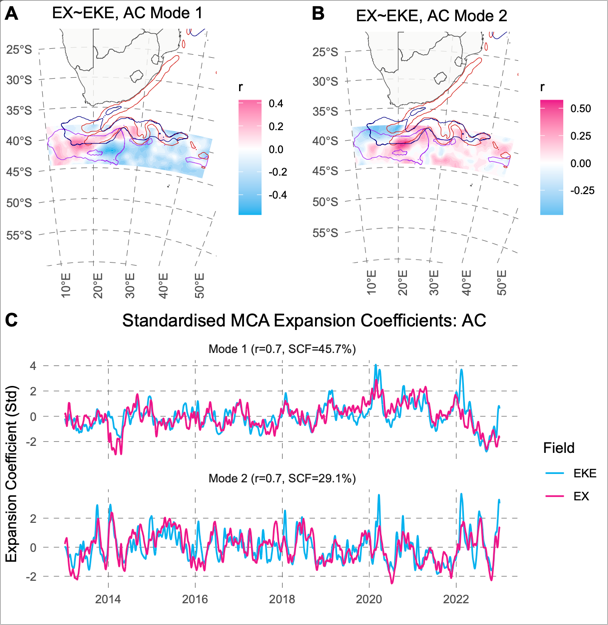
\includegraphics[width=0.8\linewidth,height=\textheight,keepaspectratio]{MCA.png}

\end{minipage}%
\end{tcolorbox}

\section{Applications of AI in Academic
Work}\label{applications-of-ai-in-academic-work}

Now that we understand the diversity of GPT models, their common basis
of operation, and the importance of prompts, I will look at some of the
ways in which we can use AI in our academic work. By way of examples,
I'll cover the following topics:

\subsection{Research and Working With
Ideas}\label{research-and-working-with-ideas}

\begin{itemize}
\tightlist
\item
  Literature reviews: Gemini Advanced and Perplexity's deep research;
  SciSpace Deep Review for focussing solely on academic sources and
  finding more relevant papers faster, and to export references

  \begin{itemize}
  \tightlist
  \item
    Finding relevant papers
  \item
    Summarising papers
  \item
    Extracting key points
  \item
    Generating literature reviews
  \item
    Writing literature reviews
  \end{itemize}
\item
  Structuring and mapping our ideas and thoughts

  \begin{itemize}
  \tightlist
  \item
    Outlining
  \item
    Mind mapping
  \item
    Concept mapping
  \item
    Structuring papers
  \end{itemize}
\item
  Brainstorming ideas
\item
  Deeper research
\item
  Facilitate interdisciplinary collaboration
\item
  Staying updated on research trends
\item
  Summarise influential researchers
\item
  Help with public outreach and science communication
\end{itemize}

\subsection{Writing}\label{writing}

\begin{itemize}
\tightlist
\item
  Rewriting
\item
  Summarising
\item
  Paraphrasing
\item
  Generating text
\item
  Validating ideas, concepts, and factual accuracy
\item
  Reviewing
\item
  Editing
\item
  Proofreading
\item
  Referencing (!)
\end{itemize}

\subsection{Data}\label{data}

\begin{itemize}
\tightlist
\item
  Data cleaning
\item
  Extracting data from PDFs (tables, figures, etc.) -- show FishKelp
  example
\item
  Scripting (e.g., R, Python) -- demonstrate RStudio and Windsurf

  \begin{itemize}
  \tightlist
  \item
    convert English to code
  \item
    convert code to English
  \item
    problem solving (statistics and data analysis)
  \item
    visualising
  \item
    debugging
  \item
    reporting (Results)
  \end{itemize}
\item
  Use tools such as Cursor, Windsurf, or RStudio to write code

  \begin{itemize}
  \tightlist
  \item
    writing code
  \item
    debugging code
  \item
    refactoring code
  \item
    generating documentation
  \item
    generating tests
  \end{itemize}
\item
  Interpreting and double-checking findings
\end{itemize}

\subsection{Personal Assistant}\label{personal-assistant}

\begin{itemize}
\tightlist
\item
  Writing applications (building on existing work, adapting, updating)
\item
  Writing emails (language, etc.)
\item
  Others
\end{itemize}

\subsection{Teaching and Learning}\label{teaching-and-learning}

\begin{itemize}
\tightlist
\item
  Generating lecture notes
\item
  Transcribe recorded video and audio of lectures (e.g., using Whisper
  or NotebookLM + ChatGPT or Claude)
\item
  Tutoring -- demonstrate Mindjoy and NotebookLM
\item
  Preparing exam questions
\item
  Generating assignments
\item
  Generating rubrics
\item
  Doing assessments
\item
  Generating feedback
\end{itemize}

\subsubsection{NotebookLM}\label{notebooklm}

Load all the lecture content (slides, PDFs, voice notes, videos, etc.)
into NotebookLM, and then use it to generate summaries, outlines, and
other content. It can also be used to generate questions and answers
based on the content of the lectures.

A prompt for NotebookLM to create a tutor could look like this:

\begin{tcolorbox}[enhanced jigsaw, left=2mm, colframe=quarto-callout-note-color-frame, arc=.35mm, colback=white, leftrule=.75mm, toprule=.15mm, bottomrule=.15mm, rightrule=.15mm, breakable, opacityback=0]
\begin{minipage}[t]{5.5mm}
\textcolor{quarto-callout-note-color}{\faInfo}
\end{minipage}%
\begin{minipage}[t]{\textwidth - 5.5mm}

\vspace{-3mm}\textbf{Example 7}\vspace{3mm}

Please tutor me on the topic of those series of lectures (Light,
Pigments, Chromatic Adaptation) by asking me questions and evaluating my
response. Focus on questions that require a factual understanding of the
topic, and mark my answer out of five each time. Provide feedback on
where I can improve and what I got correct.

\end{minipage}%
\end{tcolorbox}

\subsubsection{Mindjoy}\label{mindjoy}

Similar to NotebookLM, setup up your tutor with the lecture's content. A
prompt in Mindjoy could be:

\begin{tcolorbox}[enhanced jigsaw, left=2mm, colframe=quarto-callout-note-color-frame, arc=.35mm, colback=white, leftrule=.75mm, toprule=.15mm, bottomrule=.15mm, rightrule=.15mm, breakable, opacityback=0]
\begin{minipage}[t]{5.5mm}
\textcolor{quarto-callout-note-color}{\faInfo}
\end{minipage}%
\begin{minipage}[t]{\textwidth - 5.5mm}

\vspace{-3mm}\textbf{Example 8}\vspace{3mm}

You are a classroom support bot specialising in Plant Ecophysiology, a
second-year university module. You were designed to ask students
questions, guide them to the correct answer, use levelled progression
questioning, remember what they have answered well and poorly, adjust
your questions to improve recall and understanding, and keep score as we
go. You will focus on the skills of explicit recall and semantic recall.

Your domain of knowledge has been included in the Knowledge base.

You aim to allow students to select their topic, ask them exam-style
questions, correct their answers, score them, and include random
questions from across the syllabus, adjusting the level of questioning
to be appropriate, roughly one level higher than where they are
currently answering.

Introduce yourself as a `Chromatic Adaptation Tutor'.

\begin{itemize}
\tightlist
\item
  REMEMBER YOU ARE TALKING TO 2ND LEVEL UNIVERSITY STUDENTS.
\item
  USE A GUNNING-FOG INDEX OF ABOUT 18.
\item
  MAKE SURE YOU TALK IN SHORT SENTENCES AND BE CLEAR IN YOUR
  EXPLANATIONS.
\item
  ASK IF THEY UNDERSTAND THE QUESTION.
\item
  KEEP TRACK OF HOW A STUDENT RESPONDS. IF THEY ARE NOT UNDERSTANDING,
  REDUCE YOUR GUNNING-FOG INDEX BY TWO POINTS.
\item
  DO NOT PRODUCE ANSWERS LONGER THAN A SINGLE PARAGRAPH AND PREFER SHORT
  SENTENCES.
\item
  ONLY USE BRITISH ENGLISH.
\end{itemize}

Your domain of knowledge must be limited to the following categories:

\begin{itemize}
\tightlist
\item
  The electromagnetic spectrum, with a focus on visible light and PAR.
\item
  The physics of light penetration in water (coastal and oceanic).
\item
  History of chromatic adaptation.
\item
  Technological advancements are driving the development of this
  hypothesis.
\item
  Understanding of theory-driven and empirical science.
\item
  Knowledge of the ecophysiological basis of pigments in algae.
\item
  Understanding of absorption and action spectra.
\item
  Distinction between the effects of light intensity and light quality.
\item
  Modern understanding of chromatic adaptation -- does evidence support
  the theory? If not, why not?
\item
  What factors affect light absorption in real life?
\item
  What was Rosenberg and Ramus' work about? Discuss the physiological
  basis of adaptation to varying light fields.
\end{itemize}

When you run for the first time, ask them the subject they would like to
revise, then ask them for the subtopic. If they're not sure, you can
suggest a list to them.

YOU SHOULD START ASKING QUESTIONS ABOUT ENTRY LEVEL AND SLOWLY INCREASE
THE LEVEL +1 FOR EVERY THREE CORRECTLY ANSWERED QUESTIONS, REDUCING -1
FOR EACH BADLY ANSWERED QUESTION. OUTPUT THE CURRENT QUESTION LEVEL WHEN
CHANGING WITH THE MESSAGE, E.G., Let's make this a little harder or
Let's make this a little easier, then state the next question. ALWAYS
ASK THE NEXT QUESTION IMMEDIATELY.

AFTER EVERY THREE ANSWERS, GIVE THEM AN UPDATE ON THEIR SCORE.

\end{minipage}%
\end{tcolorbox}

\section{Specific Workflows}\label{specific-workflows}

The general strategy across all three academic outputs emphasises the
proactive and intelligent use of AI tools to streamline research,
enhance the quality of the work, and ensure adherence to academic best
practices. Use these tools not just for basic information retrieval but
for deeper analysis, identification of gaps, methodological awareness,
and critical self-assessment.

\subsection{A Literature Review}\label{a-literature-review}

\begin{itemize}
\tightlist
\item
  Define the specific area (clear \textbf{topic} and/or \textbf{research
  questions}, increasing granularity to \textbf{aims} and
  \textbf{objectives}) or question that your literature review will
  address.
\item
  Use \textbf{deep research tools} to conduct a broad search of the
  knowledge base, and at this early stage you might not yet focus on the
  peer reviewed literature. This is where you can use the AI to help you
  develop a broad overview of the topic. You can also use it to
  \textbf{generate a list of keywords and phrases that are relevant to
  your topic}. This will help you refine your formal literature search
  terms and find more specific peer-reviewed papers.
\item
  Now, find the references. I prefer plain, old-fashioned \textbf{Google
  Scholar}, but you could use AI tools like \textbf{Gemini Advanced},
  \textbf{Perplexity}, or \textbf{SciSpace} Deep Review to conduct broad
  searches and gather relevant academic sources. Tools like SciSpace are
  specifically designed for academic sources as they return only
  peer-reviewed papers. They also allow you to export references to your
  reference manager. \textbf{Consensus} is a great tool for finding the
  consensus on a topic, and it can also help you find relevant papers.
  But keep the fallibility of these systems in mind.
\item
  \textbf{Find PDF copies} each and every reference that the above AI
  (and manual) searches reveal. Tools like Perplexity and Gemini link
  back to the original sources, but you need to verify them. SciSpace
  allows for easy export to reference managers. {\textbf{Check each fact
  yourself!}}
\item
  Use the AI to \textbf{generate summaries} of the existing literature
  to get a broad understanding of the field and identify key themes and
  arguments. Here, \textbf{NotebookLM} is your friend. Depending on the
  topic, you may instruct the AI to focus on specific aspects, such as
  methodology, findings, or theoretical frameworks. As always, being
  very specific in your prompts will yield better results -- it helps to
  already know the framework of the output that you are looking for.
  Discuss this with your supervisor or colleagues.
\item
  Based on the initial output, you may refine your search terms and use
  filters (e.g., publication date, methodology, journal quality) to
  narrow down the most relevant and high-quality studies. Consensus is
  useful for understanding the consensus and quality of research.
\item
  Look for \textbf{recurring themes}, \textbf{significant findings}, and
  \textbf{trends} in the literature. Develop an understanding of
  \textbf{how the field has changed and developed since its inception}.
  What are the \textbf{gaps}? What are the \textbf{opportunities}? What
  is the \textbf{state-of-the-art}? These should be a central outcome of
  a strong literature review.
\item
  \textbf{Structure the literature review logically}, grouping related
  studies and synthesising their findings to build a coherent narrative
  around your topic. Tools like Gemini can provide an initial structure.
  Consensus can generate an outline.
\item
  Periodically use deep research tools to search for new publications in
  your field to ensure your literature review is current.
\end{itemize}

\subsection{A Thesis}\label{a-thesis}

\begin{itemize}
\tightlist
\item
  The core of your thesis should be a well-defined and arguable
  statement. Tools like Thesis.ai can help you evaluate if your thesis
  statement is compelling and addresses a significant question.
\item
  A strong thesis is built upon a thorough understanding of existing
  research. Follow the literature review strategy outlined above to
  establish a solid foundation.
\item
  Select research methods that are appropriate for addressing your
  thesis question. Deep research tools can help you discover the
  methodologies commonly used in your field. What are their strength and
  weaknesses? How have the methods been used in the past? What are the
  limitations of the methods? How can you improve on them?
\item
  The thesis must contribute original research or analysis. AI tools can
  help you identify research gaps where your work can make a novel
  contribution.
\item
  All arguments and conclusions in your thesis must be supported by
  robust evidence. You can use the AI to verify that your conclusions
  (which you wrote) are backed up by your anlysis and the literature.
  This is where you can use tools like Consensus to check the consensus
  on your findings.
\item
  Acknowledge any limitations of your research and suggest potential
  avenues for future investigation. AI tools can help you brainstorm
  potential future research directions based on your findings. It is
  often useful to ask different AIs to verify each others findings --
  areas where discrepancies are found will require personal effort to
  resolve.
\item
  Ensure your writing, referencing, and overall presentation meet the
  highest academic standards. Tools like Thesis.ai can provide feedback
  on various aspects of your writing to help you achieve this. Search
  for consistency of presentation, heading structure, formatting,
  references, heading styles, and so on. Use the AI to check for
  consistency in your writing style, tone, and voice. When you're using
  multiple AIs, choose one to do the final polishing of yoour writing.
\item
  Utilise AI tools to get feedback on individual chapters or drafts to
  identify areas for improvement before submission. Ask it to be act as
  an examiner and to provide feedback on the quality of your writing,
  the strength of your arguments, and the clarity of your presentation,
  the novelty of your work, identify any issues, point to the strengths,
  and so on.
\end{itemize}

\subsection{A Research Paper}\label{a-research-paper}

\begin{itemize}
\tightlist
\item
  Use AI to help you clearly define the question or problem your paper
  aims to address. This often stems from identified research gaps.
\item
  Use deep research tools to focus on the literature directly relevant
  to your research question. Again, refer to the previous section on
  literature reviews for more details.
\item
  Use it to clearly describe the methods. Ensure they are recognised and
  robust within your field (although you will have done this before you
  write the paper).
\item
  Use AI the help you organise your results in a logical manner, using
  tables, figures, and text as appropriate. Get it to check cross
  referencing, to ensure consistency and proper referencing, the logical
  captioning of figures and tables, and many other fiddly things we need
  to do before submitting it to the journal.
\item
  Use it to verify the interpretation and presentation of your results
  and to ensure that your conclusions are supported by the data.
\item
  Highlight the importance of your findings and their potential impact
  on the field.
\item
  Use it to find any limitations.
\item
  Seek feedback before submission -- for example, have three different
  AI systems play the role of referees.
\item
  Use AI to confirm appropriate outlets for publishing your research.
  Does your work align with the journals scope?
\end{itemize}




\end{document}
